\textbf{Beispiel 4}\\ \\
a)\\ \\
Zeichnung:
\begin{figure}[h]
	\centering
	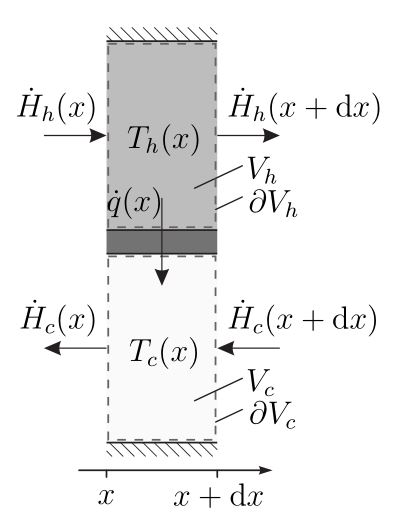
\includegraphics[width= 5cm]{tikz/13_07_2018_4a}
\end{figure}
\newline
Sämtliche Wärmeströme aus der Zeichnung lauten
\begin{align*}
	\dot{H}_h(x) &= \dot{m}_hc_pT_h(x) \\
	\dot{H}_h(x + \text{d}x) &= \dot{m}_hc_pT_h(x + \text{d}x) \\
	\dot{H}_c(x) &= \dot{m}_cc_pT_c(x) \\
	\dot{H}_c(x + \text{d}x) &= \dot{m}_cc_pT_c(x + \text{d}x) \\
	\dot{q}(x) &= kB(T_h(x) - T_c(x))
\end{align*}
b)\\ \\
Die beiden Energiebilanzen des Kontrollvolumen lauten
\begin{align*}
	\dot{m}_hc_pT_h(x) - \dot{m}_hc_pT_h(x + \text{d}x) - kB(T_h(x) - T_c(x))\text{d}x &= 0 \\
	\dot{m}_cc_pT_c(x) - \dot{m}_cc_pT_c(x + \text{d}x) - kB(T_h(x) - T_c(x))\text{d}x &= 0
\end{align*}
Durch Umformen erhält man die Differentialgleichungen
\begin{align*}
	\frac{\text{d}T_h(x)}{\text{d}t} &= \frac{kB}{\dot{m}_hc_p}\left(T_h(x) - T_c(x)\right) \\
	\frac{\text{d}T_c(x)}{\text{d}t} &= \frac{kB}{\dot{m}_cc_p}\left(T_h(x) - T_c(x)\right)
\end{align*}
c)\\ \\
Durch Lösen dieses Differentialgleichungssystem ergeben sich für die beiden Temperaturverläufe
\begin{align*}
	T_h(x) &= K \frac{T_{c,2} - T_{h,1}}{KL + 1}x + T_{h,1} \\
	T_c(x) &= T_h(x) - \frac{T_{c,2} - T_{h,1}}{KL + 1}
\end{align*}
mit
\[
	K = \frac{kB}{\dot{C}}
\]
Zu verwendende Formel zum Lösen befinden sich in der Formelsammlung. \\ \\
d)\\ \\
Mit den gegebenen Ansätzen und der Formel für den Gesamtwärmestrom eines Wärmetauschers aus der Formelsammlung folgt
\[
	\dot{Q} = kB(a - c)L
\]
e)\\ \\
Es existieren viele konstruktive Maßnahmen um den Wärmestrom zu erhöhen.Hier müssen jedoch nur zwei genannt werden.
\begin{enumerate}
	\item[i)] Erhöhung des Wärmedurchgangskoeffizienten durch Erzwingen einer turbulenten Strömung im Fluid.
	\item[ii)] Vergrößerung der Übergangsfläche durch eine größere Bauform des Wärmetauschers
\end{enumerate}